\chapter{Aplicación Web}

La aplicación web se ha creado con el objetivo de proporcionar una interfaz atractiva y manejable usada como panel de administración de forma que podamos interactuar con los cuestionarios, respuestas e información mostrada en el bot. Esta solución garantiza la integridad y el almacenamiento seguro de los datos almacenados en una base de datos centralizada. 

La aplicación web funciona como intermediario entre el usuario y el bot. Esta se encarga de la creación de cuestionarios, del procesamiento y visualización de las repuestas de manera organizada, lo que facilita su posterior análisis. Nace como solución a satisfacer la importancia de la automatización y agilidad en la recopilación de datos, logrando un enfoque integral para la administración y respuestas de usuarios.

El chatbot se ha pensado para ser utilizado por los usuarios. Sin embargo, la aplicación solo podrá ser usada por el administrador o las personas autorizadas para su uso. En este capítulo explicaré los pasos seguidos para su desarrollo.


\section{Arquitectura} 


Django es un framework basado en el modelo  MVC (Model-View-Controller). MVC es un patrón arquitectónico que separa una aplicación en tres componentes lógicos principales: el modelo, la vista y el controlador. Cada uno de estos componentes está diseñado para manejar aspectos de desarrollo específicos de una aplicación. Además, MVC es uno de los marcos de desarrollo web estándar de la industria más utilizados para crear proyectos escalables y extensibles.

Django implementa este patrón MVC de una manera peculiar y con algunas variaciones que ellos llaman MTV, que viene siendo la de Model, Template, View \textit{(\cite{djangomvt})}.

\begin{itemize}

\item M significa "Model" (Modelo), la capa de acceso a la base de datos. Esta capa contiene toda la información sobre los datos: cómo acceder a estos, cómo validarlos, cuál es el comportamiento que tiene, y las relaciones entre los datos.

\item T significa "Template" (Plantilla), la capa de presentación. Esta capa contiene las decisiones relacionadas a la presentación: como algunas cosas son mostradas sobre una página web u otro tipo de documento.

\item V significa "View" (Vista), la capa de la lógica de negocios. Esta capa contiene la lógica que accede al modelo y la delega a la plantilla apropiada: puedes pensar en esto como un puente entre el modelos y las plantillas.

\end{itemize}

Esta es la lógica seguida para el desarrollo. Si nos adentramos en el codigo, vemos que existe una carpeta llamada \textit{'applications'} que contiene varias subcarpetas y en la que cada una es una tabla diferente en la base de datos. Dentro de estas subcarpetas es donde estan creadas las operaciones relacionadas con los modelos y las vistas. En un nivel superior encontramos la carperta \textit{'templates'}, que incluye las plantillas que dan funcionalidad a estas vistas, tambien separadas por modelos. Y por último dentro de la carpeta \textit{'static'} se encuentran los archivos que dan apariencia a estas plantillas.



\section{Login}


\begin{figure}[!ht]
    \centering
    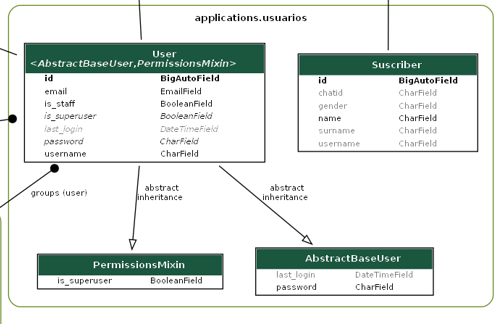
\includegraphics[width=1\textwidth, height=6.5cm]{imagenes/usuarios.png}
    \caption{ Diagrama tabla usuarios }
    \label{fig:usuarios}
\end{figure}

Existen 2 tipos de usuarios en nuestro sistema como vemos en la \textit{\hyperref[fig:usuarios]{figura 6.1}}

El primer usuario, identificado como \textit{User} que actua como administrador, y es el que cuenta con  todos los privilegios para poder acceder y modificar las tablas de la base de datos además de poder acceder al sistema. Y el segundo tipo \textit{Suscriber} que son los usuarios registrados por el bot sin ningún tipo de autoridad. 

En Django, las operaciones asociadas a los usuarios se manejan a través del sistema de autenticación que tiene incorporado. Permite manejar cuentas de usuario, grupos, permisos, inicios y cierres de sesión, reestablecimiento de contraseñas y sesiones de usuario basadas en cookies. Todo esto ya viene implementado por defecto, pero proporciona opciones para reemplazar y así ampliarlo y personalizarlo para satisfacer las necesidades de tu proyecto.

El login, que se ve en la \textit{\hyperref[fig:login]{figura 6.2}}, es la primera página que se muestra cuando intentamos entrar. Solo pueden acceder a la aplicación los usuarios registrados.

\begin{figure}[!ht]
    \centering
    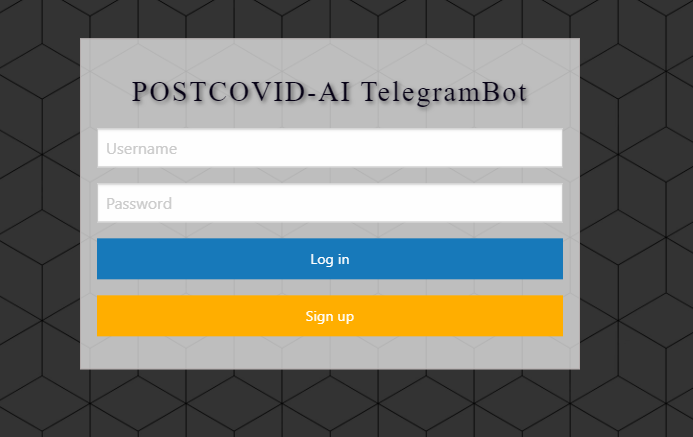
\includegraphics[width=1\textwidth]{imagenes/login.png}
    \caption{ Login usuarios }
    \label{fig:login}
\end{figure}
\vspace{0.8cm}

En caso de no estar registrado se provee de un formulario para ello como se muestra en la \textit{\hyperref[fig:general]{figura 6.3}} . Este rellena los campos de la tabla User que crea un nuevo registro de usuario en el sistema para que pueda autenticarse y acceder a él. Además otorga todos los permisos de administrador para que pueda realizar cualquier tipo de acción. \vspace{0.3cm}


\begin{figure}[!ht]
  \centering
  \begin{subfigure}{0.7\textwidth}
    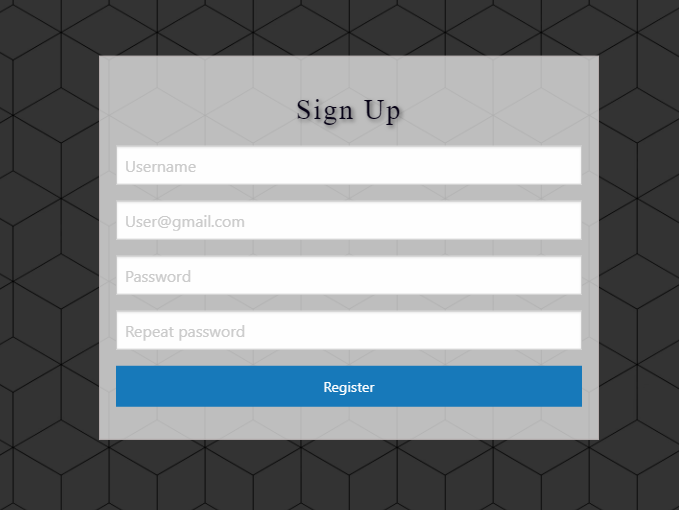
\includegraphics[width=\linewidth]{imagenes/register.png}
    \label{fig:imagen1}
  \end{subfigure}
  \hfill
  \begin{subfigure}{0.7\textwidth}
    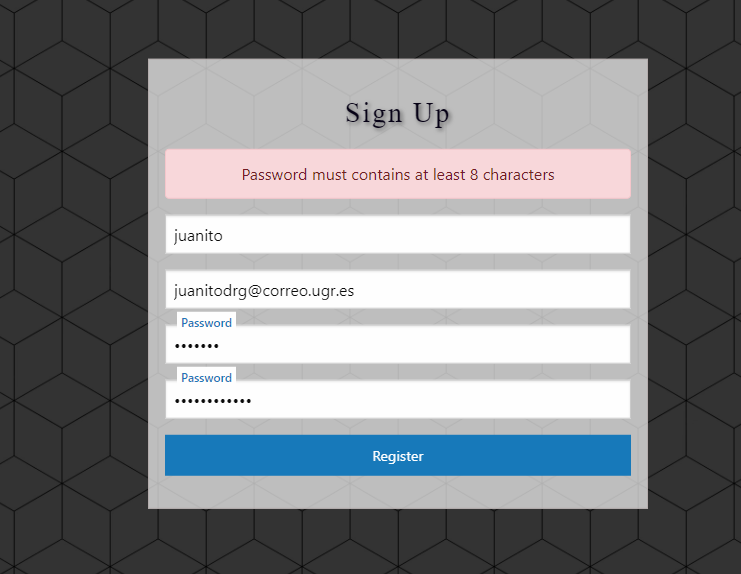
\includegraphics[width=\linewidth]{imagenes/register2.png}
    \label{fig:imagen2}
  \end{subfigure}

  \caption{Formulario de registro}
  \label{fig:general}
\end{figure}\vspace{1cm}

Cada usuario que desee registarse deberá especificar un username, email y la contraseña. El formulario cuenta con validaciones como que el nombre de usuario no se encuentre repetido en el sistema, escribir la contraseña dos veces y que coincidan o que esta tenga más de 8 caracteres. \vspace{1cm}

\section{Home}

Una vez logueados en el sistema, nos redirigirá al home. El home es la vista principal de la aplicación, la primera página que los usuarios ven cuando acceden al sitio web \textit{\hyperref[fig:home]{figura 6.4}}. Proporciona información clave y navegación a otras secciones. Este consta de 4 secciones principales: Preguntas, Bloques, Contextos, Respuestas.\vspace{0.5cm}

\begin{figure}[!ht]
    \centering
    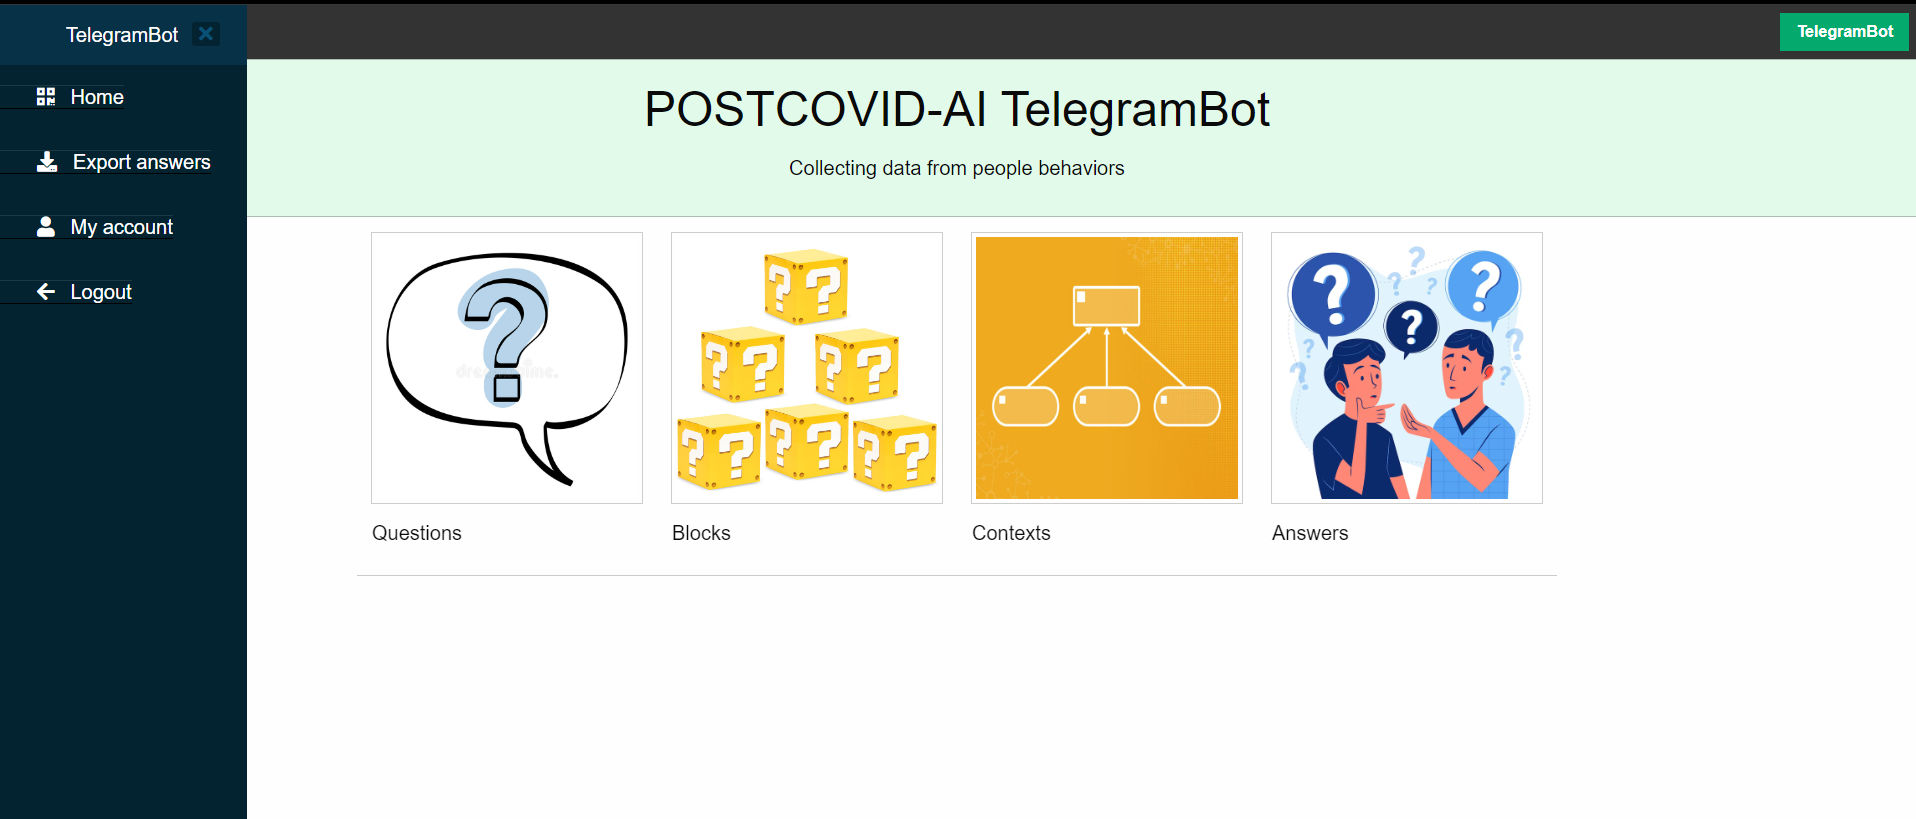
\includegraphics[width=1\textwidth, height=6cm]{imagenes/home.png}
    \caption{ Home }
    \label{fig:home}
\end{figure}
\vspace{0.5cm}

Todas las vistas además cuentan con una barra lateral desplegable para realizar algunas operaciones de manera rápida como exportar respuestas, modificar la información del usuario y hacer logout. 

\begin{figure}[!ht]
    \centering
    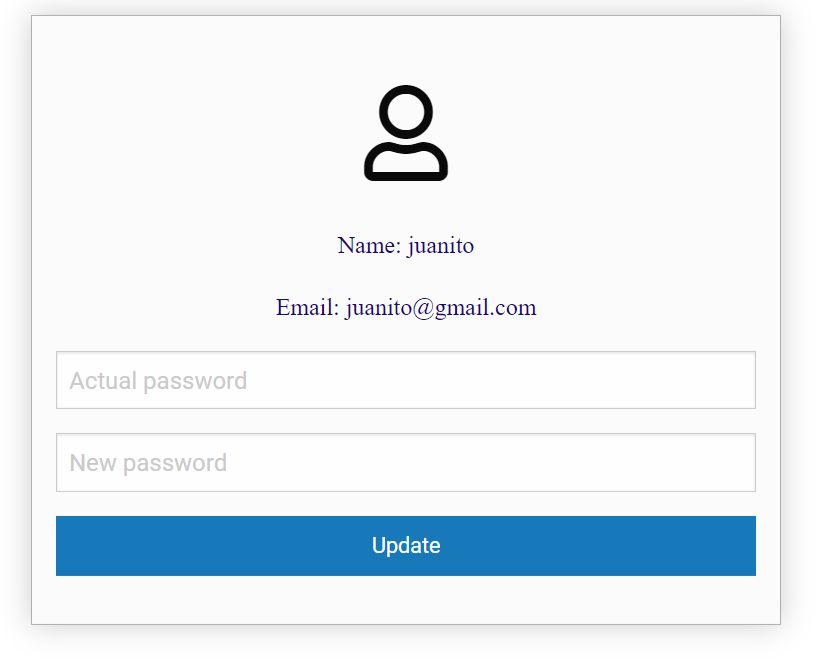
\includegraphics[width=0.5\textwidth, height=5cm]{imagenes/user_update.png}
    \caption{ Actualización usuario }
    \label{fig:modify-user}
\end{figure}

Por ejemplo, en la \textit{\hyperref[fig:modify-user]{figura 6.5}} se muestra la vista de modificar usuario donde nos muestra un formulario con los datos del usuario que se encuentra activo y nos da la posibilidad de cambiar la contraseña, pudiendo proporcionar una nueva.



\section{Gestores}


Todas las secciones que veremos consisten en tablas paginadas que muestran la información guardada de cada registro pertenecientes a cada modelo. Además todas constan de un botón para añadir un nuevo registro, eliminar y otro para modificar. \vspace{0.3cm}

Se ha implementado un buscador en cada una de las vistas de cada sección.

\begin{figure}[!ht]
    \centering
    
\includegraphics[width=0.5\textwidth]{imagenes/search.png}
    \caption{ Buscador }
    \label{fig:enter-label}
\end{figure}

Este buscador mostrará la lista de registros cuyos nombres coincidan con aquello escrito, para facilitar el acceso a la información deseada de manera más eficiente.

\subsection{Preguntas}

\begin{figure}[!ht]
    \centering
    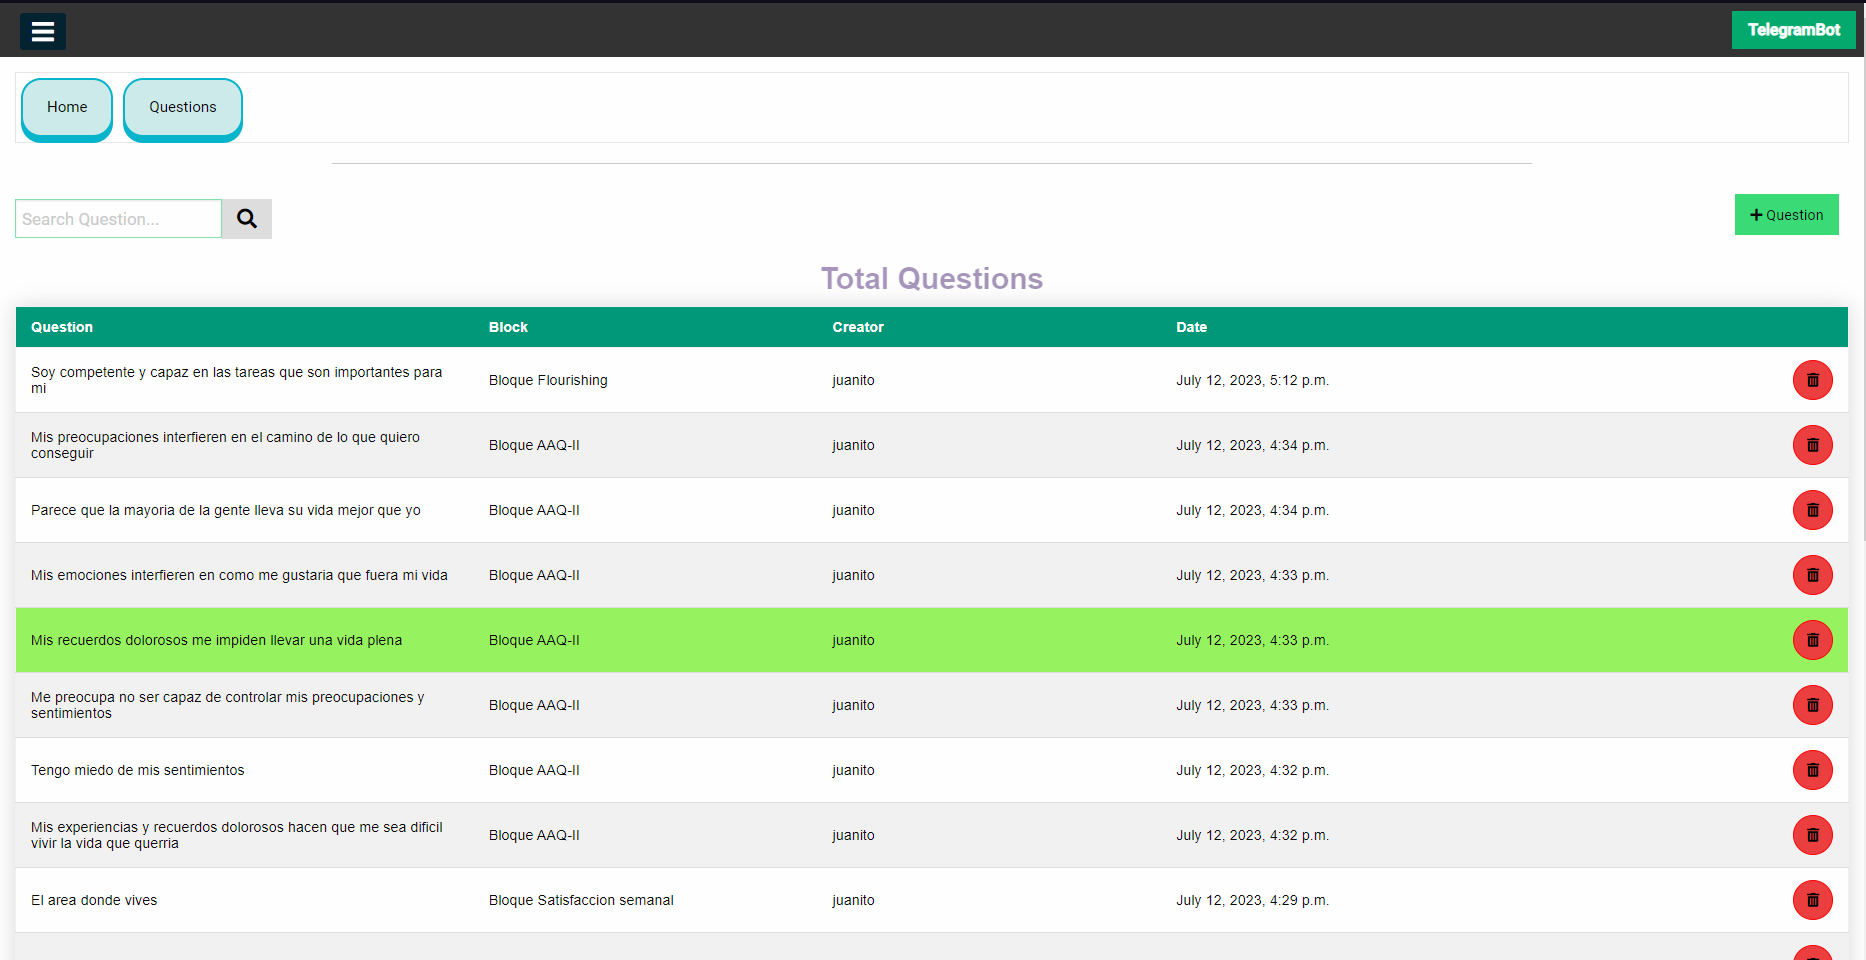
\includegraphics[width=1\textwidth]{imagenes/list_quest.png}
    \caption{ Listado de preguntas }
    \label{fig:vista-preguntas}
\end{figure}\vspace{1cm}

Dentro de la tabla de preguntas se muestra de forma general los campos mas relevantes para distinguirlas, mostrado en la \textit{\hyperref[fig:vista-preguntas]{figura 6.7}}, como el enunciado, el bloque al que pertenecen, la fecha y el usuario que la ha creado. 

Como vemos en la parte superior derecha se encuentra un botón para añadir una pregunta. Si navegamos por las filas de la tabla y clicamos en una se nos abrirá la vista para modificar la pregunta. Además en la parte derecha de cada fila hay un botón para eliminar el registro deseado. 

Si se pulsa en el botón para añadir una pregunta se abrirá una nueva página con un formulario con los datos necesarios para registrarla. 


A nivel de base de datos los campos que requiere cada pregunta son los siguientes:\vspace{0.3cm}

\begin{itemize}
    \item \textit{id}
    \item  \textit{title}: Enunciado de la pregunta.
    \item \textit{creator}: Foreign key a Usuario.
    \item \textit{date}: Fecha en la que se crea la pregunta. 
\end{itemize}\vspace{0.3cm}

El id como en todas las tablas es la clave primaria. A su vez, la pregunta tiene una clave externa a la tabla \textit{Posibles Respuestas}. Por lo que cada pregunta tiene varias posibles respuestas y cada posible respuesta tiene asignada una pregunta. En este caso, como se ve en la \textit{\hyperref[fig:add-question]{figura 6.8}}, para registrar la pregunta solo necesitamos proporcionar el titulo y las posibles respuestas ya que el campo de creador se autorellena con el usuario que la crea y la fecha se pone a la actual.\vspace{1cm}

\begin{figure}[!ht]
    \centering
    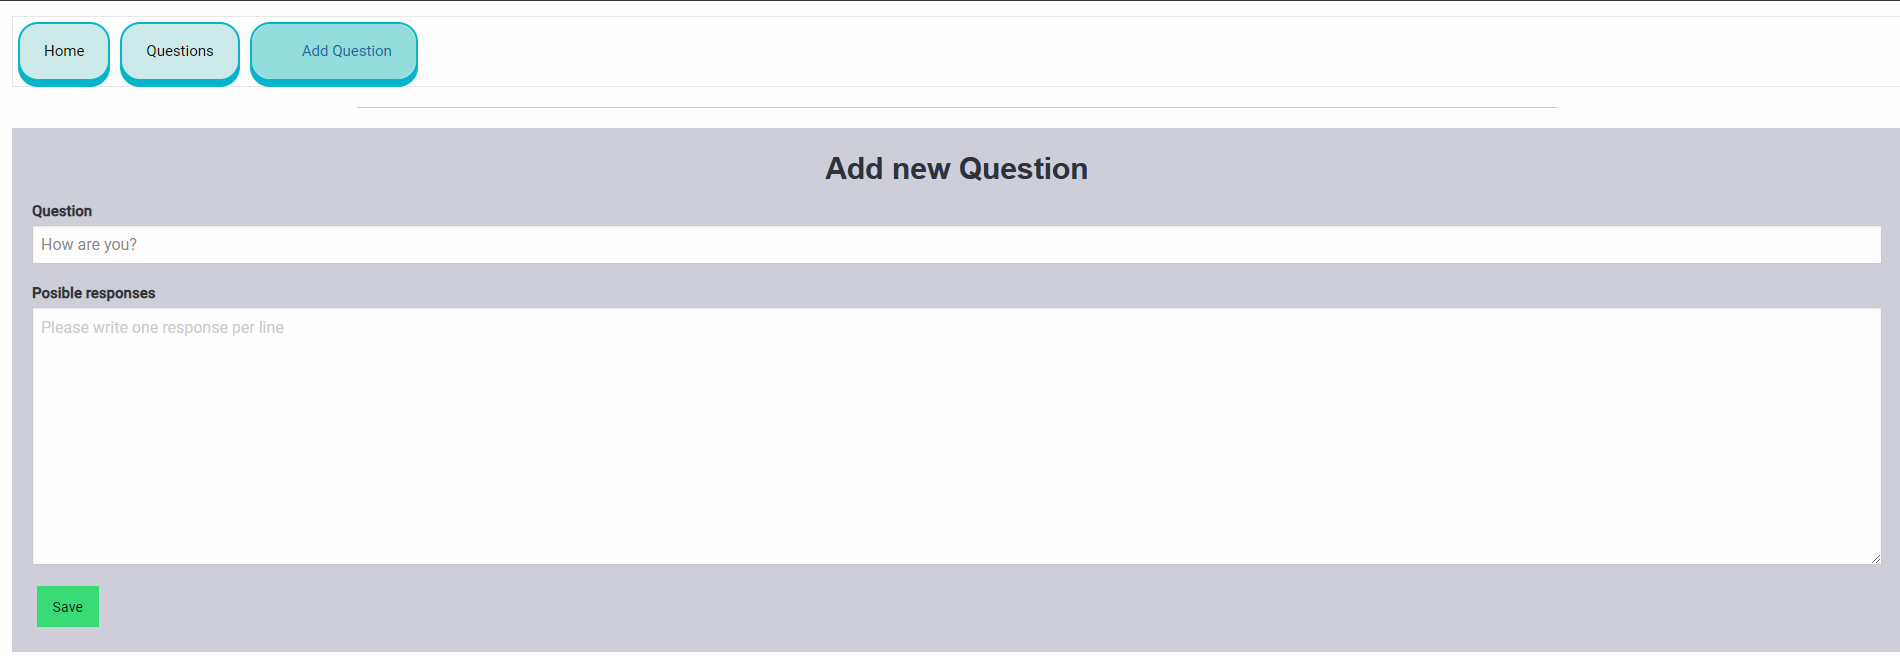
\includegraphics[width=1\textwidth]{imagenes/add_pregunta.png}
    \caption{ Añadir pregunta}
    \label{fig:add-question}
\end{figure}\vspace{1cm}

Dentro del panel de posibles respuestas debemos añadir las respuestas a esa pregunta, cada una separada por línea. A su vez cuando se cree la pregunta también se crearán los registros de las respuestas asociadas a la pregunta. \vspace{1cm}

\begin{figure}[!ht]
    \centering
    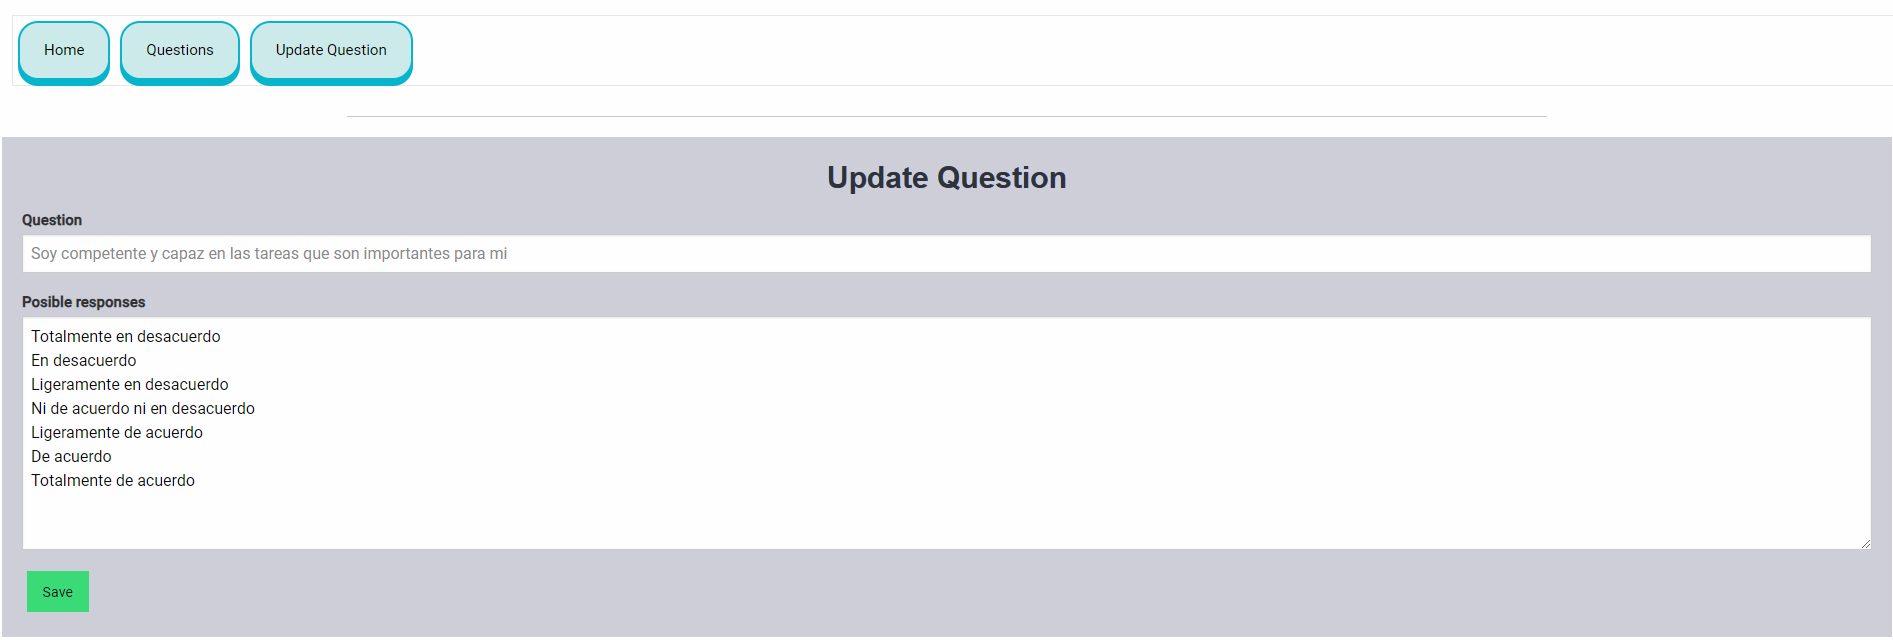
\includegraphics[width=1\textwidth]{imagenes/update_pregunta.png}
    \caption{ Modificar Pregunta}
    \label{fig:modify-question}
\end{figure}\vspace{0.5cm}

En la \textit{\hyperref[fig:modify-question]{figura 6.9}} observamos el formulario de modificación de la pregunta en el que se puede cambiar el titulo y las respuestas. Si otro usuario modifica la pregunta también se actualiza el campo del creador y fecha.

Y por último si se selecciona el botón de eliminar (que se ve como un símbolo de papelera rojo a la derecha de cada fila), aparecerá una alerta para verificar si realmente se desa borrar la pregunta \textit{\hyperref[fig:delete-question]{(figura 6.10)}}.

\begin{figure}[!ht]
    \centering
    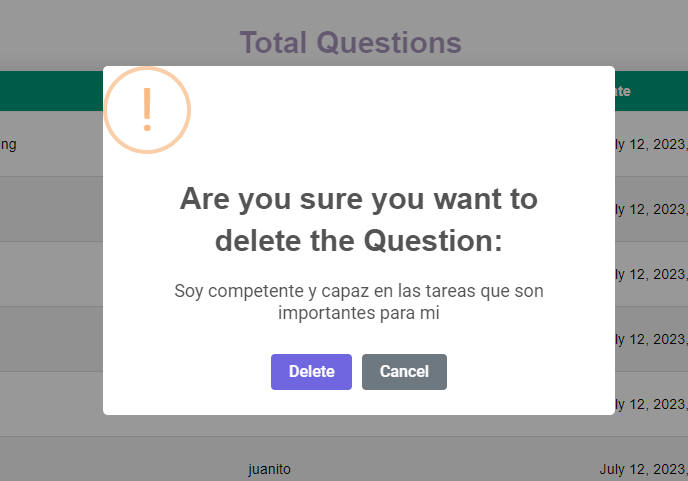
\includegraphics[width=0.7\textwidth, height=7cm]{imagenes/delete_pregunta.png}
    \caption{ Borrar Pregunta}
    \label{fig:delete-question}
\end{figure}\vspace{3cm}



\subsection{Bloques}

\begin{figure}[!ht]
    \centering
    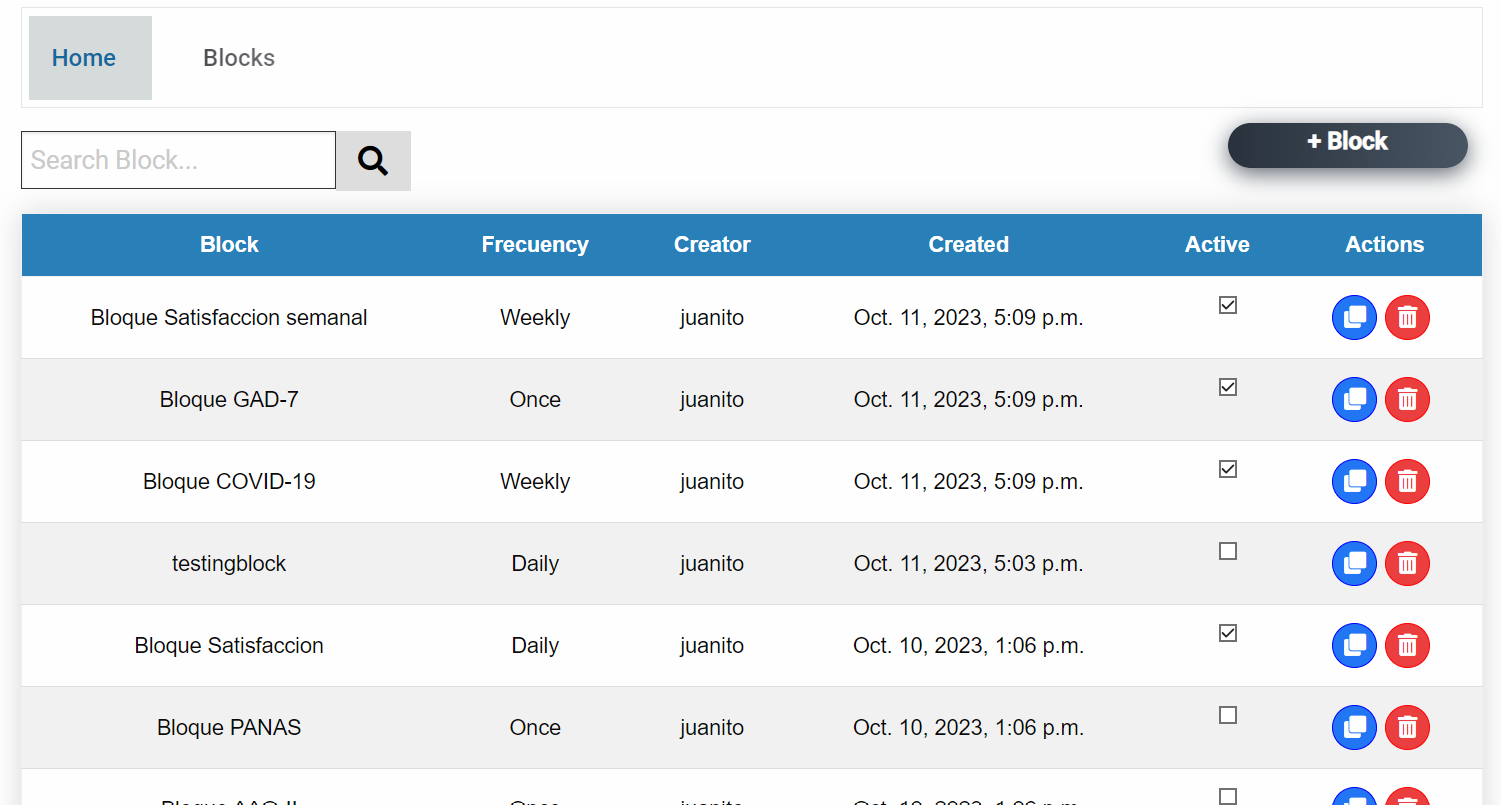
\includegraphics[width=1\textwidth]{imagenes/list_bloques.png}
    \caption{Listado de Bloques}
    \label{fig:lista-bloques}
\end{figure}\vspace{1cm}

La \textit{\hyperref[fig:lista-bloques]{figura 6.11}} muestra la tabla que contiene los registros de los bloques de preguntas en el sistema. Al igual que en la vista anterior cuenta con las operaciones de añadir, modificar y eliminar un bloque. \vspace{0.3cm}

Los campos necesarios para registrar un bloque en la base de datos son los siguientes: \vspace{0.3cm}

\begin{itemize}
    \item \textit{id}
    \item \textit{block}: nombre del bloque.
    \item \textit{active}: atributo booleano que indica si el bloque se encuentra activo.
    \item \textit{questions}: Foreign Key a pregunta.
    \item \textit{context}: Foreign key a contexto.
    \item \textit{frecuency}: Frecuencia del bloque.
    \item \textit{importance}: Importancia del bloque.
\end{itemize}\vspace{0.3cm}

El campo \textit{questions} es una relacion de tipo \textit{ManyToMany} con la tabla de preguntas. Un mismo bloque tendrá la posibilidad de asignar el número de preguntas que desee. Todas esas preguntas a su vez pertenecerán a ese bloque.  

Como vemos en la \textit{\hyperref[fig:add-bloque]{figura 6.12}}, se puede elegir mediante un checkbox las preguntas que se desee añadir y un recuadro en el que  muestra una lista de los contextos creados en el sistema, para elegir uno y asignarlo al bloque. \vspace{0.7cm}


\begin{figure}[!ht]
    \centering
    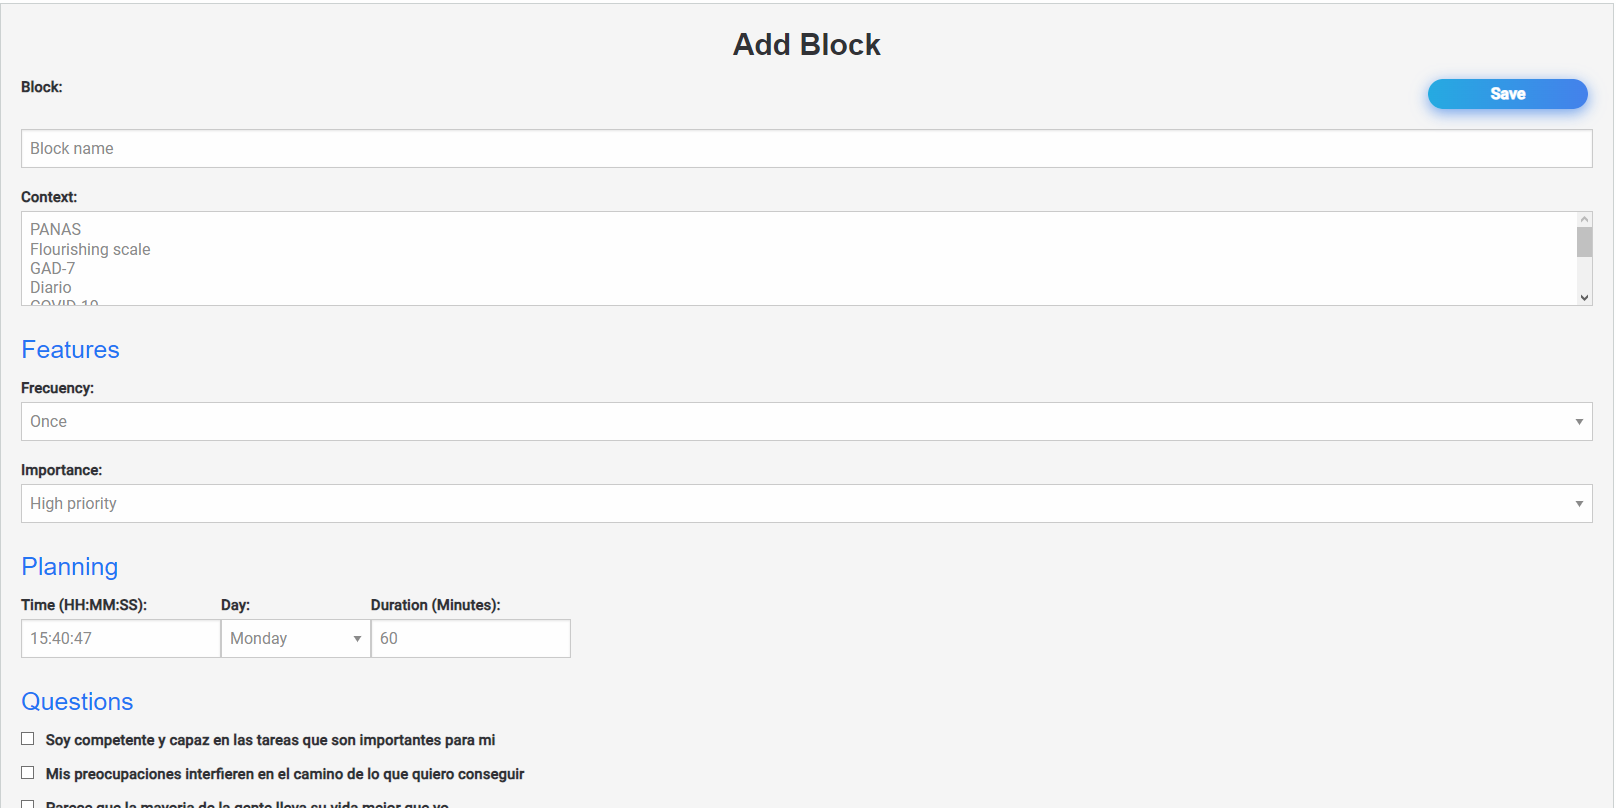
\includegraphics[width=1\textwidth]{imagenes/add_block.png}
    \caption{Añadir bloque}
    \label{fig:add-bloque}
\end{figure}\vspace{0.7cm}

Una vez se han añadido preguntas al bloque y se le ha asignado un contexto, faltaría definir la frecuencia del bloque y su importancia. Estos atributos están más relacionados con el bot. La frecuencia define cada cuanto tiempo se debe realizar el cuestionario asociado al bloque. Normalmente, las preguntas dentro de un mismo bloque tienen un sentido y un propósito común. Por ejemplo, hay preguntas sobre salud, horas de sueño, alimentación que necesitan de realizarse todos los días o una vez por semana. Mientras que hay otras que con solo hacerse una vez ya bastaría. De ahí nace la idea de agrupar las preguntas en bloques. Dentro de la frecuencia puede elegir entre:

\begin{itemize}
    \item Once
    \item Daily
    \item Weekly
    \item Monthly
\end{itemize}

Y como último campo la importancia del bloque (High importance, Normal, Low importance). Este campo  se añadió para que a la hora de que el bot haga el cuestionario de un bloque, priorice los de mayor importancia ante los otros.

\subsection{Contextos}

Los contextos contienen los mensajes a mostrar por parte del bot en el chat del usuario cuando se va a tratar un tema concreto. Cuando se entra en un bloque el bot muestra un mensaje a forma de introducción que nos pone en contexto acerca del tema a tratar en el cuestionario. Esta tabla se crea como idea para que haya variedad a la hora de mostrar estos mensajes introductorios. \vspace{0.7cm}

\begin{figure}[!ht]
    \centering
    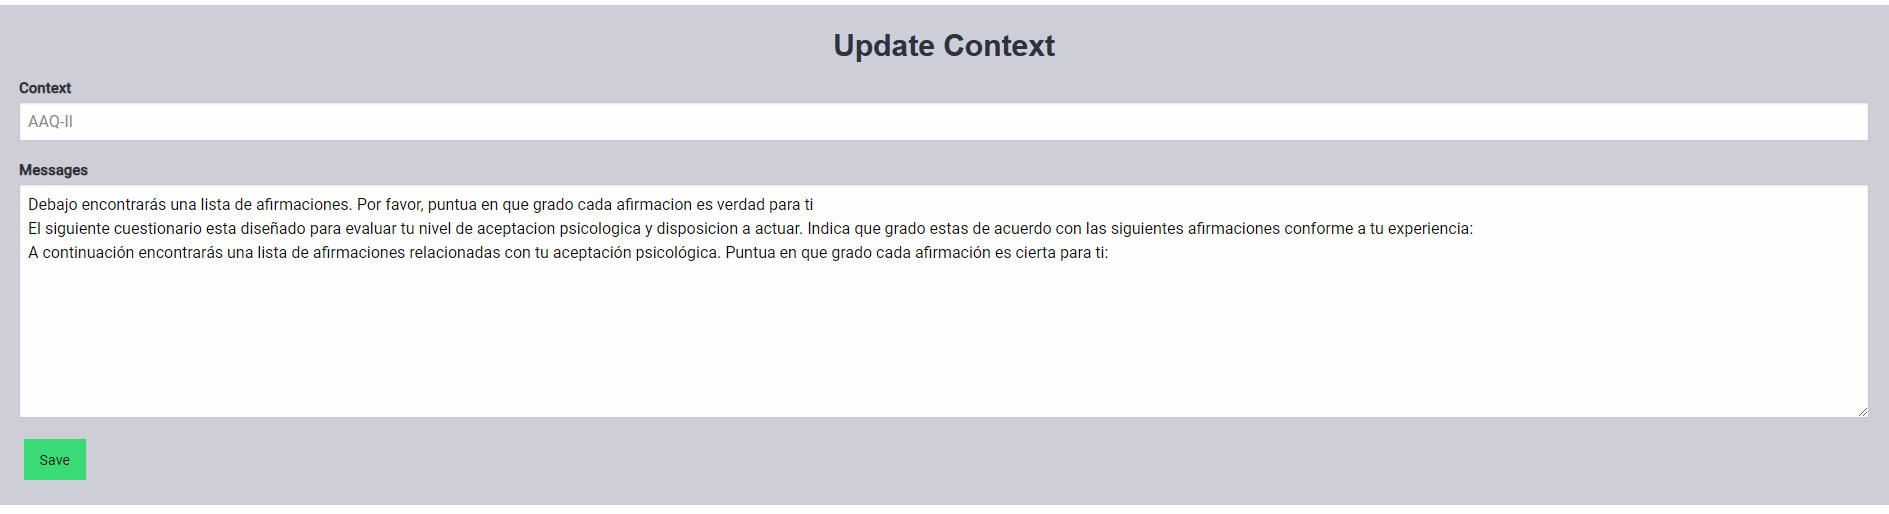
\includegraphics[width=1\textwidth]{imagenes/update_context.png}
    \caption{Editar bloque}
    \label{fig:update-bloque}
\end{figure}\vspace{0.7cm}

En la \textit{\hyperref[fig:update-bloque]{figura 6.13}} se puede ver un ejemplo que nos aclara con mayor detalle la función del contexto. El tema es AAQ-II, estas preguntas sirve para evaluar el nivel de aceptación psicológica y disposición a actuar de una persona. Cuando se realice el cuestionario asociado se mostrará uno de los tres mensajes que dispone. 

La forma de crearlos es parecida a la de las preguntas que se explica previamente. Existen 2 tablas: \textit{Contextos} y \textit{Mensajes}. La clase contexto contiene los nombres, y la de mensajes los enunciados de la información a mostrar, que tienen una clave foránea a contexto. 

\textbf{Clase Contexto:}

\begin{itemize}
    \item \textit{name}: Nombre.
\end{itemize}

\textbf{Clase Mensaje}

\begin{itemize}
    \item \textit{text}: Enunciado del mensaje.
    \item \textit{context}: Foreign key a Contexto.
\end{itemize}


Para crearlo se especifica el nombre y los mensajes, cada uno separado por una línea, que crea todos los registros y los asocia al contexto actual.\vspace{0.5cm}

\subsection{Respuestas}

Por último nos encontramos el apartado de respuestas, mostrado en la \textit{\hyperref[fig:list-answers]{figura 6.14}}. Esta vista es simplemente a modo de visualización ya que el administrador no podrá realizar operaciones con ellas. Estas se crean automáticamente cuando un usuario responde a la pregunta hecha por el bot. \vspace{1cm}

\begin{figure}[!ht]
    \centering
    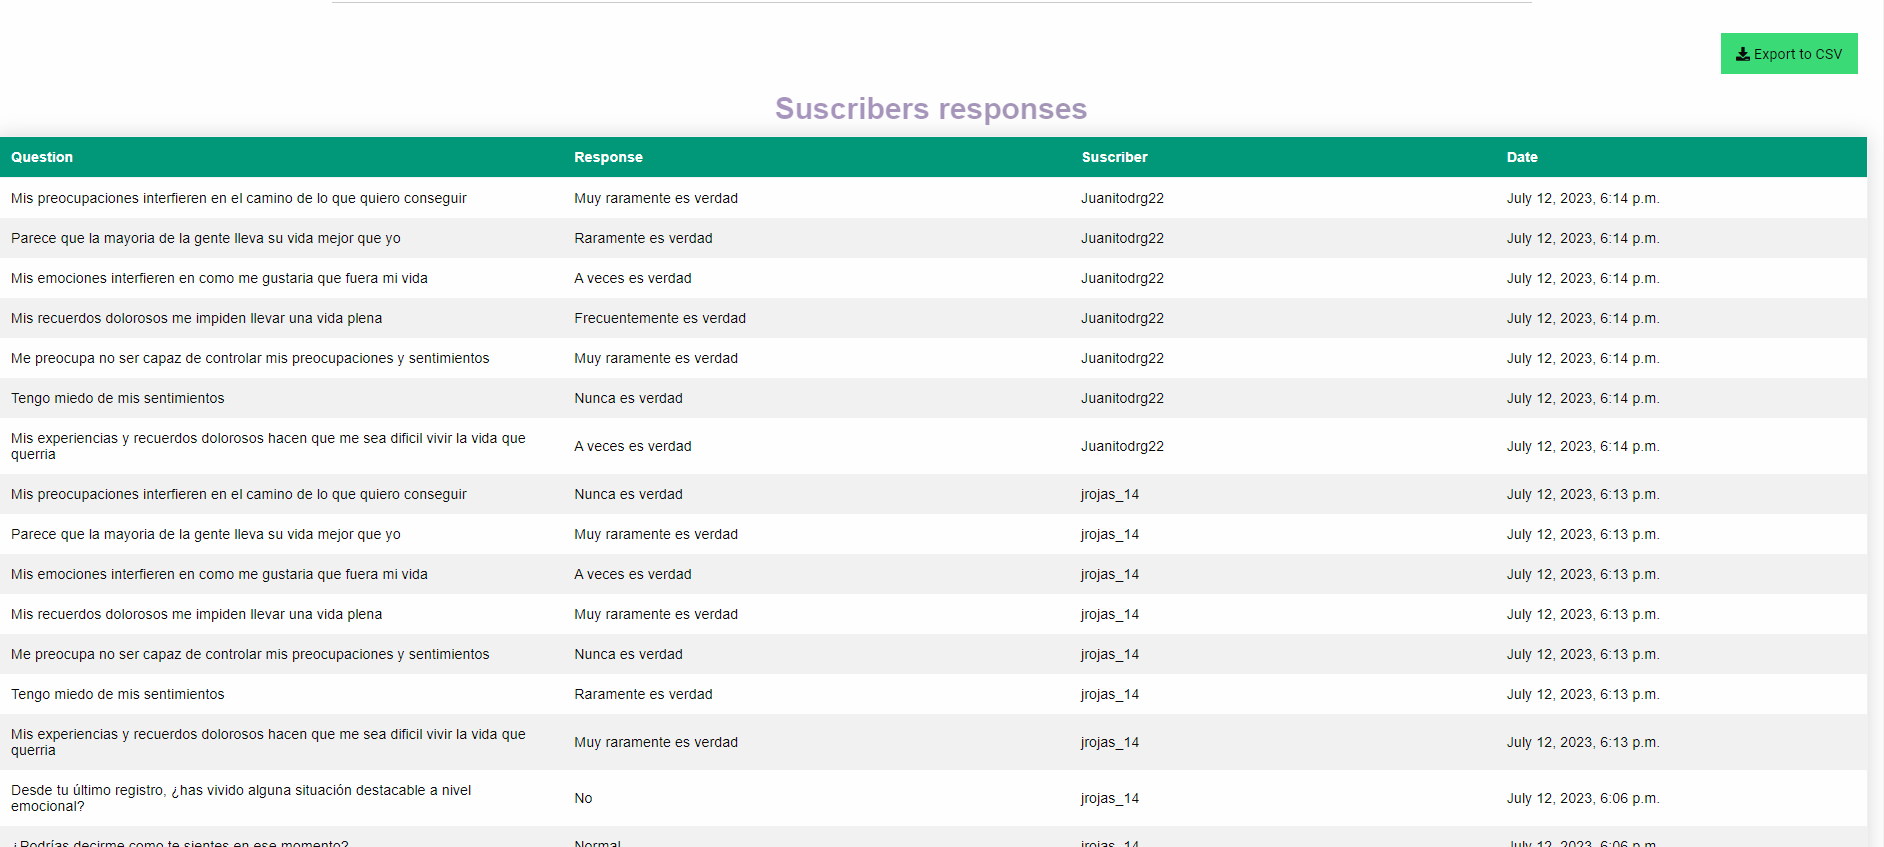
\includegraphics[width=1\textwidth]{imagenes/list_answers.png}
    \caption{Lista respuestas}
    \label{fig:list-answers}
\end{figure}\vspace{0.5cm}



Los campos para registar una respuesta son los siguientes:

\begin{itemize}
    \item \textit{id}
    \item \textit{question}: Foreign key a pregunta.
    \item \textit{response}: Respuesta del usuario.
    \item \textit{suscriber}: Foreign key a usuario.
    \item \textit{date}: Fecha de la respuesta.
\end{itemize}

Esta vista cuenta además con un botón en la parte superior derecha para exportar las respuestas a formato CSV. Los archivos CSV almacenan los datos separados con comas, por lo que cuando se guarda el texto y los números es fácil moverlos de un programa a otro. Al fin y al cabo este es el propósito de nuestro proyecto, recaudar información y entregarla en un formato específico para que el análisis sea sencillo.\vspace{1cm} 

La función que lo realiza es la siguiente:

\begin{lstlisting}[language=Python]
def export_to_csv(request):
    answers = Answer.objects.all()
    response = HttpResponse('text/csv')
    response['Content-Disposition'] = 'attachment; filename=answers_export.csv'
    writer = csv.writer(response)
    writer.writerow(['Question', 'Response', 'Suscriber', 'Date'])
    answer_fields = answers.values_list('question__title', 'response', 'suscriber__username', 'date')
    for answer in answer_fields:
        writer.writerow(answer)
    return response
\end{lstlisting}

Python cuenta con una librería llamada csv. Esta librería implementa clases para leer y escribir datos tabulados en formato CSV.